\documentclass[
]{jss}

\usepackage[utf8]{inputenc}

\providecommand{\tightlist}{%
  \setlength{\itemsep}{0pt}\setlength{\parskip}{0pt}}

\author{
Jorge Cimentada\\Max Planck Insitute for Demographic Research \And Wiebke Weber\\Pompeu Fabra University
}
\title{\pkg{measurementerror}: A flexible tool to correct correlation and
covariance matrices for measurement error}

\Plainauthor{Jorge Cimentada, Wiebke Weber}
\Plaintitle{measurementerror: A flexible tool to correct correlation and covariance
matrices for measurement error}
\Shorttitle{\pkg{measurementerror}: measurement error correction}

\Abstract{
The abstract of the article.
}

\Keywords{\proglang{R}, measurement error}
\Plainkeywords{R, measurement error}

%% publication information
%% \Volume{50}
%% \Issue{9}
%% \Month{June}
%% \Year{2012}
%% \Submitdate{}
%% \Acceptdate{2012-06-04}

\Address{
    Jorge Cimentada\\
  Max Planck Insitute for Demographic Research\\
  First line Second line\\
  E-mail: \email{cimentadaj@demogr.mpg.de}\\
  
    }

% Pandoc header

\usepackage{amsmath}

\begin{document}

\hypertarget{introduction}{%
\section{Introduction}\label{introduction}}

Here we introduce the problem and the package. This should indicate *
The substantive problem: the literature on measurement error and why
this has been a problem (Wiebke) * The theoretical work by the person
who devised what we implement in the package (Wiebke) * A brief
comparison to existing software in the R programming language (Jorge) *
A description of the software we introduce to fix the problem (Jorge)

Packages to check out for Jorge:

\url{https://cran.csiro.au/web/packages/mmc/mmc.pdf}
\url{https://cran.r-project.org/web/packages/eivtools/eivtools.pdf}
\url{https://rdrr.io/cran/brms/man/me.html}
\url{https://cran.r-project.org/web/packages/GLSME/GLSME.pdf}

This section should be around a page or so

\hypertarget{literature-on-measurement-error}{%
\section{Literature on measurement
error}\label{literature-on-measurement-error}}

This section should describe the three type of corrections that the
package implements. This brief part should introduce the general reader
to measurement error literature and the type of measurement errors
techniques which are available and their limitations.

The sections below should contain the images and formulas that describe
the methods we implement making references to the authors who
implemented each one. I've written down three subsection for each
implementation but feel free to change anything you think should be
changed. Since this is a statistical software journal, it's ok to go
full in swing with formulas.

Citations can be written like this: Blah blah
\citetext{\citealp[see][pp.~33-35]{alwin2007}; \citealp[also][ch.~1]{scherpenzeel1997}}.
Blah blah \citep[pp.~33-35, 38-39 and \emph{passim}]{alwin2007}. Blah
blah \citep{alwin2007, scherpenzeel1997}.

\hypertarget{correction-for-simple-concepts}{%
\subsection{Correction for simple
concepts}\label{correction-for-simple-concepts}}

Any image can be saved in the folder figs/ and just copy the code below
replacing the name of image from below

\begin{CodeChunk}


\begin{center}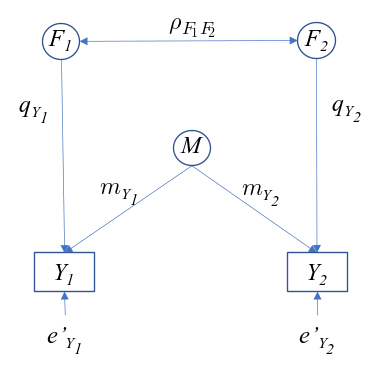
\includegraphics[width=0.5\linewidth]{figs/simpleconcepts} \end{center}

\end{CodeChunk}

\hypertarget{correction-for-simple-concepts-with-complex-concepts}{%
\subsection{Correction for simple concepts with complex
concepts}\label{correction-for-simple-concepts-with-complex-concepts}}

\begin{CodeChunk}


\begin{center}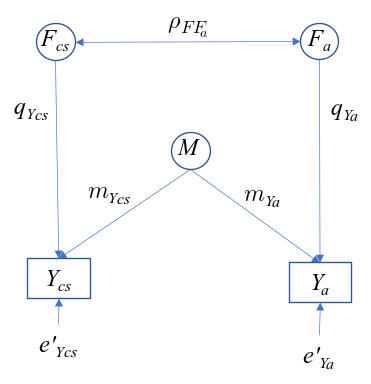
\includegraphics[width=0.5\linewidth]{figs/simplecomplex} \end{center}

\end{CodeChunk}

\hypertarget{correct-for-complex-concepts-and-complex-concepts}{%
\subsection{Correct for complex concepts and complex
concepts}\label{correct-for-complex-concepts-and-complex-concepts}}

\begin{CodeChunk}


\begin{center}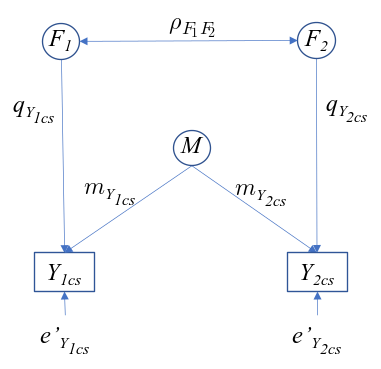
\includegraphics[width=0.5\linewidth]{figs/complexcomplex} \end{center}

\end{CodeChunk}

\hypertarget{applications-and-illustrations}{%
\section{Applications and
illustrations}\label{applications-and-illustrations}}

Here we should have 1 example that illustrates the three descriptions
from above. Or, N number of examples showing how to use the methods
described above. These should be fairly simply examples (if more than 1)
or one single example which elaborates in complexity.

From looking at several papers online, I think it might be better to
focus on one example and begin with something simple: only correct for
quality, then CMV, the simple concepts vs complex concepts and finalize
with complex vs complex concepts. Otherwise it's too difficult (at least
for me) to find several examples that we can use all of the
applications.

\hypertarget{political-trust-example}{%
\subsection{Political Trust example}\label{political-trust-example}}

In this case study we will go through an applied example of the
capabilities of the \texttt{measurementfree} package.

We'll begin by loading some packages we'll use.

\begin{CodeChunk}

\begin{CodeInput}
R> library(lavaan)
\end{CodeInput}

\begin{CodeOutput}
This is lavaan 0.6-3
\end{CodeOutput}

\begin{CodeOutput}
lavaan is BETA software! Please report any bugs.
\end{CodeOutput}

\begin{CodeInput}
R> library(dplyr)
\end{CodeInput}

\begin{CodeOutput}

Attaching package: 'dplyr'
\end{CodeOutput}

\begin{CodeOutput}
The following objects are masked from 'package:stats':

    filter, lag
\end{CodeOutput}

\begin{CodeOutput}
The following objects are masked from 'package:base':

    intersect, setdiff, setequal, union
\end{CodeOutput}

\begin{CodeInput}
R> library(ggplot2)
R> library(essurvey)
\end{CodeInput}

\begin{CodeOutput}

Please cite as: 
\end{CodeOutput}

\begin{CodeOutput}
Cimentada, Jorge (2019). Download Data from the European Social Survey on the Fly R package version 1.0.2.
\end{CodeOutput}

\begin{CodeInput}
R> library(sqpr)
R> library(magrittr)
R> 
R> # And measurementfree
R> library(measurementfree)
\end{CodeInput}

\begin{CodeOutput}

Please cite as: 
\end{CodeOutput}

\begin{CodeOutput}
Cimentada, J. & Weber, W. (2019). A flexible tool to correct correlation and covariance matrices for measurement error R package version 0.0.1.
\end{CodeOutput}
\end{CodeChunk}

\hypertarget{read-the-data}{%
\subsection{Read the data}\label{read-the-data}}

Let's read in the data from the European Social Survey using the
\texttt{essurvey} package and create a sum score of a number of
variables. A sum score is the weighted \((w)\) \texttt{sum} of a number
of variables \((y_1, y_2, ..., y_k)\) to create a composite score
\((CS)\):

Be sure to register at the Europen Social Survey website and run
\texttt{set\_email("your\_email@email.com")} replacing the fake email
with your registered one.

\begin{CodeChunk}

\begin{CodeInput}
R> # Choose your selected variables
R> selected_vars <- c("trstprl", "trstplt", "trstprt",
R+                    "stfedu", "stfhlth", "psppsgv",
R+                    "psppipl", "ptcpplt", "ppltrst",
R+                    "polintr", "stflife", "stfeco",
R+                    "agea", "eisced")
R> 
R> # Download the ESS data and clear missing values
R> ess7es <- import_country("Spain", 7, "cimentadaj@gmail.com")[c(selected_vars, "pspwght")]
\end{CodeInput}

\begin{CodeOutput}
Downloading ESS7
\end{CodeOutput}

\begin{CodeInput}
R> ess7es <- ess7es[complete.cases(ess7es), ]
R> 
R> # Calculate the standardized but unweighted sums cores
R> 
R> ess7es <-
R+   within(ess7es, {
R+     poltrst <- scale(trstprl) + scale(trstplt) + scale(trstprt)
R+     serv <- scale(stfedu) + scale(stfhlth)
R+     systmrsp <- scale(psppsgv) + scale(psppipl) + scale(ptcpplt)
R+   })
R> 
R> # Calculate the standard deviation of each sum score
R> w_pol <- 1 / sd(ess7es$poltrst)
R> w_serv <- 1 / sd(ess7es$serv)
R> w_systmrsp <- 1 / sd(ess7es$systmrsp)
R> 
R> # Create the weighted and standardized composite score
R> ess7es <-
R+   within(ess7es, {
R+     poltrst <- w_pol*scale(trstprl) + w_pol*scale(trstplt) + w_pol*scale(trstprt)
R+     serv <- w_serv*scale(stfedu) + w_serv*scale(stfhlth)
R+     systmrsp <- w_systmrsp*scale(psppsgv) + w_systmrsp*scale(psppipl) + w_systmrsp*scale(ptcpplt)
R+   })
R> 
R> composite_scores <- c("poltrst", "serv", "systmrsp")
R> 
R> all_vars <- c(composite_scores, selected_vars) # for later use
\end{CodeInput}
\end{CodeChunk}

So far we have the original \texttt{tibble} with a few extra columns
containing the composite sum scores:

\begin{CodeChunk}

\begin{CodeInput}
R> ess7es
\end{CodeInput}

\begin{CodeOutput}
# A tibble: 1,624 x 18
   trstprl trstplt trstprt  stfedu stfhlth psppsgv psppipl ptcpplt  ppltrst
   <dbl+l> <dbl+l> <dbl+l> <dbl+l> <dbl+l> <dbl+l> <dbl+l> <dbl+l> <dbl+lb>
 1 0 [No ~ 0 [No ~ 1 [1]   3 [3]   1 [1]   3 [3]   0 [Not~ 0 [Not~  6 [6]  
 2 5 [5]   4 [4]   4 [4]   3 [3]   5 [5]   5 [5]   6 [6]   3 [3]    6 [6]  
 3 4 [4]   3 [3]   3 [3]   3 [3]   8 [8]   6 [6]   2 [2]   4 [4]    7 [7]  
 4 3 [3]   0 [No ~ 3 [3]   2 [2]   2 [2]   0 [Not~ 0 [Not~ 0 [Not~ 10 [Mos~
 5 0 [No ~ 0 [No ~ 0 [No ~ 0 [Ext~ 2 [2]   0 [Not~ 1 [1]   5 [5]    7 [7]  
 6 0 [No ~ 0 [No ~ 0 [No ~ 0 [Ext~ 0 [Ext~ 0 [Not~ 0 [Not~ 0 [Not~  2 [2]  
 7 5 [5]   0 [No ~ 0 [No ~ 5 [5]   3 [3]   0 [Not~ 2 [2]   0 [Not~  5 [5]  
 8 4 [4]   0 [No ~ 0 [No ~ 5 [5]   4 [4]   0 [Not~ 0 [Not~ 0 [Not~  3 [3]  
 9 5 [5]   0 [No ~ 0 [No ~ 8 [8]   5 [5]   0 [Not~ 0 [Not~ 0 [Not~  0 [You~
10 0 [No ~ 0 [No ~ 0 [No ~ 0 [Ext~ 0 [Ext~ 0 [Not~ 0 [Not~ 1 [1]    1 [1]  
# ... with 1,614 more rows, and 9 more variables: polintr <dbl+lbl>,
#   stflife <dbl+lbl>, stfeco <dbl+lbl>, agea <dbl+lbl>, eisced <dbl+lbl>,
#   pspwght <dbl>, systmrsp[,1] <dbl>, serv[,1] <dbl>, poltrst[,1] <dbl>
\end{CodeOutput}
\end{CodeChunk}

Let's read in the SQP data. The Survey Quality Predictor (SQP) database
contains the quality information of thousands of questions. We can
access this database with the \texttt{sqpr} package. To do that, you'll
need to register with the SQP (\href{www.sqp.upf.edu}{sqp.upf.edu}) and
then we can login with \texttt{sqp\_login()} using your valid SQP
credentials:

\begin{CodeChunk}

\begin{CodeInput}
R> sqp_login("your user name", "your password")
\end{CodeInput}
\end{CodeChunk}

Once that's done, we can continue accessing the data.

\begin{CodeChunk}

\begin{CodeInput}
R> me_data <-
R+   get_sqp(
R+     study = "ESS Round 7",
R+     question_name = selected_vars[1:12],
R+     country = "ES",
R+     lang = "spa"
R+   )
\end{CodeInput}
\end{CodeChunk}

Let's confirm all of our questions were extracted.

\begin{CodeChunk}

\begin{CodeInput}
R> me_data
\end{CodeInput}

\begin{CodeOutput}
# A tibble: 12 x 4
   question reliability validity quality
   <chr>          <dbl>    <dbl>   <dbl>
 1 ppltrst        0.737    0.952   0.702
 2 polintr        0.624    0.964   0.601
 3 psppsgv        0.766    0.927   0.709
 4 psppipl        0.762    0.928   0.707
 5 ptcpplt        0.766    0.928   0.711
 6 trstprl        0.812    0.959   0.779
 7 trstplt        0.852    0.965   0.822
 8 trstprt        0.858    0.956   0.821
 9 stflife        0.721    0.911   0.657
10 stfeco         0.797    0.912   0.727
11 stfedu         0.757    0.838   0.635
12 stfhlth        0.76     0.798   0.607
\end{CodeOutput}
\end{CodeChunk}

Why are we only selecting 12 of our 14 variables? You'll see later on.
We will add the measurement quality of the last two manually because
they're not in the SQP database.

\hypertarget{analysis}{%
\subsection{Analysis}\label{analysis}}

With the function \texttt{me\_sscore} we can calculate the quality of a
sum score. Remember those sum scores we calculated at the beginning? We
can calculate the quality of the sum score by specifying the data from
the SQP API, the data from the European Social Survey and provide
\texttt{me\_sscore} with the variables that contribute to the sum score.

For example, this code..

\begin{CodeChunk}

\begin{CodeInput}
R> me_sscore(me_data = me_data,
R+           .data = ess7es,
R+           new_name = poltrst,
R+           trstprl, trstplt, trstprt)
\end{CodeInput}

\begin{CodeOutput}
# A tibble: 10 x 4
   question reliability validity quality
   <chr>          <dbl>    <dbl>   <dbl>
 1 ppltrst        0.737    0.952   0.702
 2 polintr        0.624    0.964   0.601
 3 psppsgv        0.766    0.927   0.709
 4 psppipl        0.762    0.928   0.707
 5 ptcpplt        0.766    0.928   0.711
 6 stflife        0.721    0.911   0.657
 7 stfeco         0.797    0.912   0.727
 8 stfedu         0.757    0.838   0.635
 9 stfhlth        0.76     0.798   0.607
10 poltrst       NA       NA       0.912
\end{CodeOutput}
\end{CodeChunk}

creates a new variable called \texttt{poltrst} which will have the
quality of the sum score of \texttt{trstprl}, \texttt{trstplt},
\texttt{trstprt}. Note that these three variables are \textbf{not}
present anymore, but only \texttt{poltrst}, the summary of the three.
For our analysis we want to repeat that for the three sum scores from
the beginning. Let's extend it:

\begin{CodeChunk}

\begin{CodeInput}
R> quality <-
R+   me_data %>%
R+   me_sscore(ess7es, new_name = poltrst, trstprl, trstplt, trstprt) %>%
R+   me_sscore(ess7es, new_name = serv, stfedu, stfhlth) %>%
R+   me_sscore(ess7es, new_name = systmrsp, psppsgv, psppipl, ptcpplt)
\end{CodeInput}
\end{CodeChunk}

Let's see how it looks like.

\begin{CodeChunk}

\begin{CodeInput}
R> quality
\end{CodeInput}

\begin{CodeOutput}
# A tibble: 7 x 4
  question reliability validity quality
  <chr>          <dbl>    <dbl>   <dbl>
1 ppltrst        0.737    0.952   0.702
2 polintr        0.624    0.964   0.601
3 stflife        0.721    0.911   0.657
4 stfeco         0.797    0.912   0.727
5 poltrst       NA       NA       0.912
6 serv          NA       NA       0.750
7 systmrsp      NA       NA       0.842
\end{CodeOutput}
\end{CodeChunk}

Great! We have our summarized \texttt{tibble}. Sometimes you'll want to
manually append predictions such as quality estimates not available in
the SQP API. For our case, we want to add the \texttt{quality} estimates
of the variables \texttt{agea} and \texttt{eised} (remember those two we
were excluding from before? we were excluding them because they're not
available in the SQP data base). For that we can use
\texttt{me\_bind\_metrics}.

\begin{CodeChunk}

\begin{CodeInput}
R> quality <-
R+   quality %>%
R+   me_bind_metrics(agea, list(quality = 1)) %>%
R+   me_bind_metrics(eisced, list(quality = 0.93))
R> 
R> quality
\end{CodeInput}

\begin{CodeOutput}
# A tibble: 9 x 4
  question reliability validity quality
  <chr>          <dbl>    <dbl>   <dbl>
1 ppltrst        0.737    0.952   0.702
2 polintr        0.624    0.964   0.601
3 stflife        0.721    0.911   0.657
4 stfeco         0.797    0.912   0.727
5 poltrst       NA       NA       0.912
6 serv          NA       NA       0.750
7 systmrsp      NA       NA       0.842
8 agea          NA       NA       1    
9 eisced        NA       NA       0.93 
\end{CodeOutput}
\end{CodeChunk}

Note that \texttt{me\_bind\_metrics} is very strict, it accepts an
\texttt{me} data frame (given by \texttt{sqpr::get\_sqp}) and it will
match that the names of your estimates (\texttt{quality} here) matches
exactly the same names in the SQP API. You can read more about it in
\texttt{?me\_bind\_metrics}. Finally, let's order our results.

\begin{CodeChunk}

\begin{CodeInput}
R> variables_order <- c("poltrst",
R+                      "serv",
R+                      "systmrsp",
R+                      "ppltrst",
R+                      "polintr",
R+                      "stflife",
R+                      "stfeco",
R+                      "agea",
R+                      "eisced")
R> 
R> quality <- quality[match(variables_order, quality$question), ]
\end{CodeInput}
\end{CodeChunk}

Briefly, let's also select these variables for ESS data.

\begin{CodeChunk}

\begin{CodeInput}
R> ess7escorr <- ess7es[c(variables_order, "pspwght")]
\end{CodeInput}
\end{CodeChunk}

\hypertarget{correlations-and-correcting-for-measurement-error}{%
\subsection{Correlations and correcting for measurement
error}\label{correlations-and-correcting-for-measurement-error}}

Let's get the correlation of all the variables in the ESS data.

\begin{CodeChunk}

\begin{CodeInput}
R> # Exploratory correlation matrix (in order of the columns in data frame):
R> original_corr_2 <- cor(ess7escorr, use = "complete.obs", method = "pearson")
R> original_corr_2
\end{CodeInput}

\begin{CodeOutput}
              poltrst        serv    systmrsp     ppltrst       polintr
poltrst   1.000000000  0.42042189  0.60203327  0.18768642 -0.2014219670
serv      0.420421888  1.00000000  0.31633682  0.11142522 -0.0212754857
systmrsp  0.602033274  0.31633682  1.00000000  0.17999428 -0.2361902279
ppltrst   0.187686419  0.11142522  0.17999428  1.00000000 -0.1987630767
polintr  -0.201421967 -0.02127549 -0.23619023 -0.19876308  1.0000000000
stflife   0.135837000  0.18062375  0.14358248  0.14719373 -0.0407515829
stfeco    0.434821138  0.38457746  0.34605350  0.09057548 -0.1050462717
agea      0.035019520  0.01604983  0.01144204 -0.05888371  0.0002020306
eisced   -0.016453690 -0.05828007  0.05296626  0.16991291 -0.3124573975
pspwght   0.007210406 -0.06471818  0.01940722  0.11507178 -0.1442207091
             stflife      stfeco          agea      eisced      pspwght
poltrst   0.13583700  0.43482114  0.0350195196 -0.01645369  0.007210406
serv      0.18062375  0.38457746  0.0160498326 -0.05828007 -0.064718182
systmrsp  0.14358248  0.34605350  0.0114420397  0.05296626  0.019407217
ppltrst   0.14719373  0.09057548 -0.0588837086  0.16991291  0.115071778
polintr  -0.04075158 -0.10504627  0.0002020306 -0.31245740 -0.144220709
stflife   1.00000000  0.27002646 -0.0375443228  0.07276395  0.021942844
stfeco    0.27002646  1.00000000  0.0165999850  0.03815190 -0.012278518
agea     -0.03754432  0.01659999  1.0000000000 -0.22553987 -0.193861040
eisced    0.07276395  0.03815190 -0.2255398662  1.00000000  0.494724370
pspwght   0.02194284 -0.01227852 -0.1938610399  0.49472437  1.000000000
\end{CodeOutput}
\end{CodeChunk}

\texttt{measurementfree} has a very similar function to \texttt{cor} but
allows to replace the diagonal and weight the correlation. In our
analysis we can use it to multiply the diagonal with the quality
estimates of all the variables and use the \texttt{pspwght} from the
European Social Survey.

\begin{CodeChunk}

\begin{CodeInput}
R> me_design <- medesign("~ stfeco + stflife",
R+                       ess7es[variables_order],
R+                       quality)
\end{CodeInput}
\end{CodeChunk}

It's the same correlation coefficients but with the diagonal set to the
quality of the estimates. But \textbf{note} that both the order of the
variables \texttt{Quality} and the order of the variables in
\texttt{ess7corr} should be the same! Otherwise we might confuse quality
estimates between variables.

For variables which are measured with the same method, we want to
account for their Common Method Variance (CMV). The
\texttt{measurementfree} package makes this very easy using the
\texttt{me\_cmv\_cor} function. Supply the correlation data frame, the
\texttt{Quality} dataset with quality estimates and
\texttt{me\_cmv\_cor} estimates the CMV between the variables specified
(here only two) and subtracts it from the correlation.

\begin{CodeChunk}

\begin{CodeInput}
R> corrected_corr <- me_cmv_cor(me_design)
\end{CodeInput}
\end{CodeChunk}

Here we have a corrected matrix for both measurement error and for the
common method variance of some variables. We can dump this into our
\texttt{sem} models and get estimates corrected for measurement error.

\hypertarget{regression-model}{%
\subsection{Regression model}\label{regression-model}}

\begin{CodeChunk}

\begin{CodeInput}
R> model <- "poltrst ~ ppltrst + stflife + polintr + stfeco + serv + systmrsp + agea + eisced"
R> 
R> # Model based on original correlation matrix
R> fit <-
R+   sem(model,
R+       sample.cov=original_corr_2,
R+       sample.nobs= 1624)
R> 
R> # Model based on corrected correlation matrix
R> corrected_corr <- as.data.frame(corrected_corr)
R> rownames(corrected_corr) <- corrected_corr$rowname
R> corrected_corr$rowname <- NULL
R> 
R> fit.corrected <-
R+   sem(model,
R+       sample.cov=as.matrix(corrected_corr),
R+       sample.nobs= 1624)
\end{CodeInput}
\end{CodeChunk}

Let's look at how much the coefficients differ

\begin{CodeChunk}

\begin{CodeInput}
R> coef_table <-
R+   list(fit, fit.corrected) %>%
R+   lapply(parameterestimates) %>%
R+   lapply(function(.x) .x[.x$lhs == "poltrst", ]) %>%
R+   lapply(function(.x) .x[c("rhs", "est", "ci.lower", "ci.upper")]) %>%
R+   do.call(rbind, .)
R> 
R> coef_table$model <- rep(c("original", "corrected"), each = 9)
R> 
R> coef_table %>%
R+   ggplot(aes(rhs, est, colour = model)) +
R+   geom_linerange(aes(ymin = ci.lower, ymax = ci.upper), position = position_dodge(width = 0.5)) +
R+   geom_point(position = position_dodge(width = 0.5)) +
R+   labs(x = "Predictors", y = "Estimated coefficients") +
R+   theme_bw()
\end{CodeInput}


\begin{center}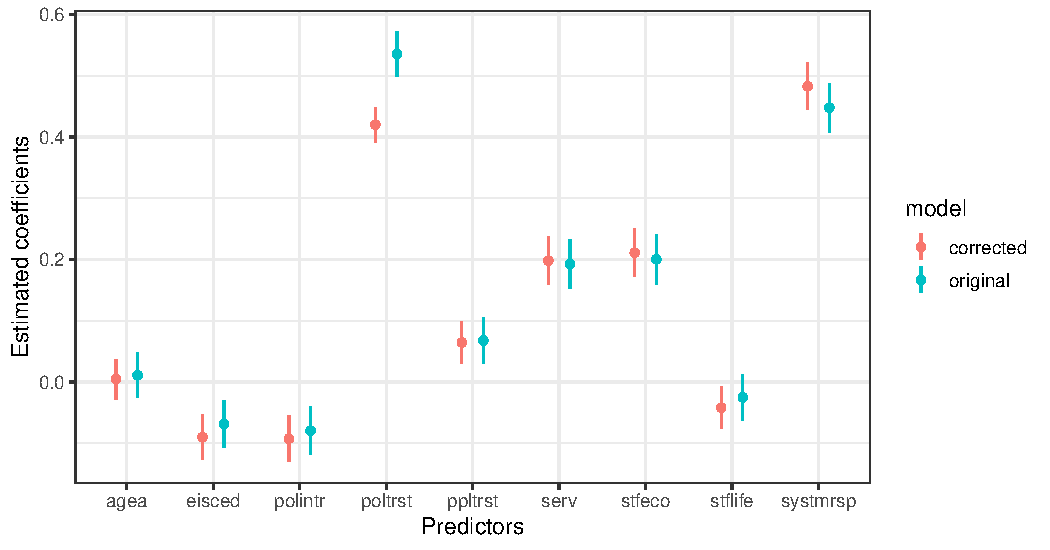
\includegraphics{measurementerror_paper_files/figure-latex/unnamed-chunk-21-1} \end{center}

\end{CodeChunk}

It differs slightly between models (although strongly for the dependent
variable). Another approach is getting the ratio between the corrected
over the original model.

\begin{CodeChunk}

\begin{CodeInput}
R> # Relative increase (they don't only go up!):
R> coef(fit.corrected) / coef(fit)
\end{CodeInput}

\begin{CodeOutput}
 poltrst~ppltrst  poltrst~stflife  poltrst~polintr   poltrst~stfeco 
           0.952            1.665            1.166            1.052 
    poltrst~serv poltrst~systmrsp     poltrst~agea   poltrst~eisced 
           1.027            1.078            0.400            1.313 
poltrst~~poltrst 
           0.785 
\end{CodeOutput}
\end{CodeChunk}

It looks like the results do differ substantially! Otherwise everything
would be at \texttt{1}.

Moreover, the R-squares of the models differ quite substantially.

\begin{CodeChunk}

\begin{CodeInput}
R> R2_uncorr <- inspect(fit, 'r2')
R> R2 <- inspect(fit.corrected, 'r2')
R> 
R> # Change of R2:
R> R2 - R2_uncorr
\end{CodeInput}

\begin{CodeOutput}
poltrst 
  0.115 
\end{CodeOutput}
\end{CodeChunk}

\hypertarget{summary}{%
\section{Summary}\label{summary}}

\hypertarget{acknowledgments}{%
\section{Acknowledgments}\label{acknowledgments}}

Everyone we acknowledge and funding

\hypertarget{computational-details}{%
\section{Computational details}\label{computational-details}}

Version for packages we used, R version, operating system

\renewcommand\refname{References}
\bibliography{bibliography.bib}


\end{document}

